\section{DATA DESCRIPTION}
The dataset\cite{palechor2019dataset} contains information on individuals from countries of Mexico, Peru, and Colombia based on their living habits and physical condition. It consists of 17 attributes and 2111 records, labeled with
\textbf{NObesity}(Obesity Level), Insufficient Weight, Normal Weight, Overweight Level I, Overweight Level II, Obesity Type I, Obesity Type II and Obesity Type III. The initial collection had 485 records, which only occupied 23\% of the full dataset. These data were labeled using Mass body index($MBI$):
$$MBI = \frac{Weight}{height^2}$$

Objects falling in different intervals of values of $MBI$ are labeled with different \textbf{NObesity} according to the definition from WHO and Mexican Normativity\cite{lanorma}. \\
After the above process, figure \ref{Fig:Data1} shows that the dataset shows unbalance with the categories of Obesity levels: most of the instances are labeled as normal weight, while relatively fewer instances are labeled as the other classes, however, the more important class in the study of obesity. This property is not good for traditional classifiers, since they tend to classify all the data into the majority class, which is less important\cite{kotsiantis2006handling}. Thus, the author generated remains 77\% of the data using the tool Weka and the filter SMOTE\cite{chawla2002smote}. Finally, the final result with 2111 records is balanced as shown in figure \ref{Fig:Data2}.

\begin{figure}[!htb]
\centering
   \begin{minipage}{0.9\textwidth}
     \centering
     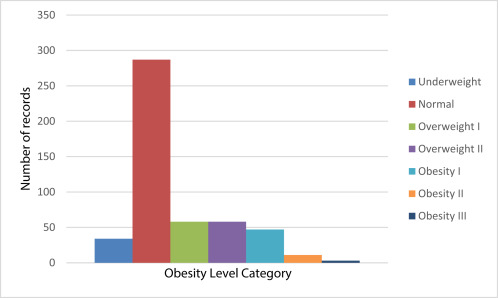
\includegraphics[width=1\linewidth]{image/rawdata.jpg}
     \caption{Unbalanced distribution of data regarding the obesity levels category.\cite{palechor2019dataset}}\label{Fig:Data1}
   \end{minipage}\hfill
   \\
   \begin{minipage}{0.9\textwidth}
     \centering
     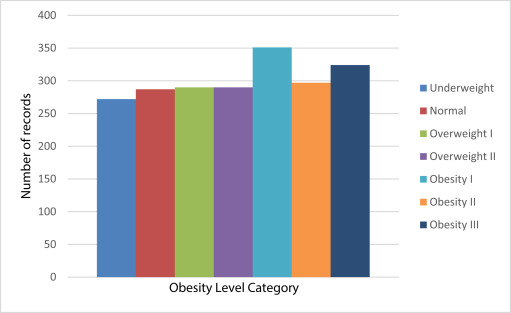
\includegraphics[width=1\linewidth]{image/balanced data.jpg}
     \caption{Balanced distribution of data regarding the obesity levels category.\cite{palechor2019dataset}}\label{Fig:Data2}
   \end{minipage}
\end{figure}

Both categorical data and numeric data are included in the dataset. Categorical features are \textbf{Gender}(Female/Male), \textbf{family history with overweight}(No/Yes), \textbf{FAVC}: Frequent consumption of high-caloric food (No/Yes), \textbf{CAEC}: Consumption of food between meals(no/sometimes/frequently/always), \textbf{SMOKE }(No/Yes),\textbf{ SCC}: Calories consumption monitoring(No/Yes), \textbf{CALC}:Consumption of alcohol(no/sometimes/frequently/always) and\textbf{ MTRANS}: Transportation used (Walking/Bike/Motorbike/Public Transportation/Automobile); numeric features are \textbf{Age}, \textbf{Height}(m), \textbf{Weight}(kg), \textbf{FCVC}:Frequency of consumption of vegetables(1-3),\textbf{ NCP}: Number of main meals(1-4), \textbf{CH2O}:Consumption of water daily(1-3), \textbf{FAF}: Physical activity frequency (0-3) and \textbf{TUE}: Time using technology devices(0-2).


